% !TeX spellcheck = en_GB_oxendict
\documentclass[11pt,a4paper]{article}
\usepackage[utf8]{inputenc}
\usepackage[T1]{fontenc}
\usepackage{amsmath,amssymb,makeidx,graphicx,float,indentfirst,color,hyperref,tikz,
	pgfplots,verbatim,fancyvrb,caption,subcaption,physics,longtable,mathrsfs, mathtools}
\numberwithin{equation}{section}
\usepackage[width=15.00cm, height=23.00cm]{geometry}
\setlength{\parindent}{4mm}
\setlength{\parskip}{1mm}
\hypersetup{colorlinks=true, linktoc=all, linkcolor=blue,}
\pgfplotsset{compat=1.15}
%\usepgfplotslibrary{groupplots,dateplot,arrows}
\usetikzlibrary{patterns,shapes.arrows}
\usepackage{listings,xcolor}
\definecolor{codegreen}{rgb}{0,0.6,0}
\definecolor{codegray}{rgb}{0.5,0.5,0.5}
\definecolor{codepurple}{rgb}{0.58,0,0.82}
\definecolor{backcolour}{rgb}{0.95,0.95,0.92}
\lstdefinestyle{mystyle}{
	backgroundcolor=\color{backcolour},   
	commentstyle=\color{codegreen},
	keywordstyle=\color{magenta},
	numberstyle=\tiny\color{codegray},
	stringstyle=\color{codepurple},
	basicstyle=\ttfamily\footnotesize,
	breakatwhitespace=false,         
	breaklines=true,                 
	captionpos=b,                    
	keepspaces=true,                 
	numbers=left,                    
	numbersep=5pt,                  
	showspaces=false,                
	showstringspaces=false,
	showtabs=true,                  
	tabsize=2,
}
\lstset{style=mystyle}
%----------------------------------------------------------------------

\author{Pritish Karmakar}

\begin{document}
	%\iffalse\fi
	\begin{titlepage}
		\pagenumbering{roman}
		\vspace*{3.5cm}
		\centering
		{\Huge\bfseries Summer Project}\\
		\vspace{5cm}
		
\includegraphics[width=2.5cm]{iiserk.png}

		\vspace{5cm}
		
		{\LARGE Pritish Karmakar\\}
		\vspace{0.3cm}
		{21MS179}
		\vfill
		
		
		\clearpage
		\tableofcontents
		\clearpage
		\listoffigures
		\listoftables
		\lstlistoflistings
		
	\end{titlepage}

\pagenumbering{arabic}

\section{POLARIZATION}

\subsection{Introduction}

\subsection{Jones formalism}
\subsubsection{Jones Vector}
Vector form of electric field of fully polarized EM wave propagating along z-axis is given by
\begin{align}
	\textbf{E}(\textbf{x},t)=
	\begin{bmatrix}
		E_x(\textbf{x},t)\\
		E_y(\textbf{x},t)\\
		E_z(\textbf{x},t)
	\end{bmatrix} =
\begin{bmatrix}
	A_x(\textbf{x}) e^{-i(kz-\omega t-\delta_x)}\\
	A_y(\textbf{x}) e^{-i(kz-\omega t-\delta_y)}\\
	0
\end{bmatrix}=
\begin{bmatrix}
	A_x(\textbf{x})e^{i\delta_x}\\
	A_y(\textbf{x})e^{i\delta_y}\\
	0
\end{bmatrix}e^{-i(kz-\omega t)}
\end{align}

We define normalized\footnote{normalized as $\textbf{J}\:\textbf{J}^\ast=1$} \textit{Jones vector} as
\begin{align}
	\textbf{J}(\textbf{x},t)=\frac{1}{\sqrt{A_x^2+A_y^2}}
	\begin{bmatrix}
		A_x(\textbf{x})e^{i\delta_x}\\
		A_y(\textbf{x})e^{i\delta_y}
	\end{bmatrix}
\end{align}

Such examples of usual polarization states are given below \cite{jones},
\begin{table}[H]
	\centering
	\begin{tabular}{ c c } 
		\hline
		\hline
		Polarization state & \textbf{J}\\
		\hline
		$\ket{H}$ & $\begin{bmatrix}1\\0\end{bmatrix}$ \\ \hline
		$\ket{V}$ & $\begin{bmatrix}0\\1\end{bmatrix}$ \\ \hline
		$\ket{P}$ & $\frac{1}{\sqrt{2}}\begin{bmatrix}1\\1\end{bmatrix}$ \\ \hline
		$\ket{M}$ & $\frac{1}{\sqrt{2}}\begin{bmatrix}1\\-1\end{bmatrix}$ \\ \hline
		$\ket{L}$ & $\frac{1}{\sqrt{2}}\begin{bmatrix}1\\i\end{bmatrix}$ \\ \hline
		$\ket{R}$ & $\frac{1}{\sqrt{2}}\begin{bmatrix}1\\-i\end{bmatrix}$ \\ 
		\hline
		\hline
	\end{tabular}
	\caption{Jones vector of usual polarization state}
	\label{table:1}
\end{table}

Some properties of Jones vector are
\begin{enumerate}
	\item The intensity of the EM wave is given by 
	\begin{align}
		I= \frac{1}{2}c\epsilon_0(A_x^2+A_y^2) = \frac{1}{2}c\epsilon_0 (E^\ast E)
	\end{align}
	\item For general elliptically polarized light we can measure the azimuth ($\alpha$) ellipticity ($\epsilon$) of the polarization ellipse by comparing Jones vector $\textbf{J}$ with \cite{WO}
	\begin{align*}
		\begin{bmatrix}
			\cos\alpha\cos\epsilon- i \sin\alpha\sin\epsilon \\
			\sin\alpha\cos\epsilon- i \cos\alpha\sin\epsilon
		\end{bmatrix}
	\end{align*}
\end{enumerate}

\subsubsection{Jones Matrix \& evolution of Jones vector}
\textit{Jones matrix} is a $2\times2$ matrix assigned for a particular optical element. Let $\textbf{M}$ be the Jones matrix for an optical element \textit{s.t.} 
\begin{align*}\textbf{M}=
	\begin{bmatrix}
		m_{11} & m_{12}\\
		m_{21} & m_{22}
	\end{bmatrix}
\end{align*}
then if a polarized light of Jones vector $\textbf{J}_{in}$ passes through that optical element then the Jones vector of output light is given by 
\begin{align}
	\textbf{J}_{out}&=\textbf{M}\;\textbf{J}_{in}\label{eq:1.4}\\	\Rightarrow \textbf{E}_{out}&=\textbf{M}\;\textbf{E}_{in} \label{eq:1.5}
\end{align}

To determine $m_{ij}$ in $\textbf{M}$,
\begin{enumerate}
	\item Pass x-polarized light and determine $\textbf{J}_{out}$, then 
	\begin{align*}
		\textbf{J}_{out}=
		\begin{bmatrix}
			m_{11} & m_{12}\\
			m_{21} & m_{22}
		\end{bmatrix}
		\begin{bmatrix}
			1\\
			0
		\end{bmatrix}=
	\begin{bmatrix}
		m_{11}\\
		m_{21}
	\end{bmatrix}
	\end{align*}

\item Pass y-polarized light and determine $\textbf{J}_{out}$, then 
\begin{align*}
	\textbf{J}_{out}=
	\begin{bmatrix}
		m_{11} & m_{12}\\
		m_{21} & m_{22}
	\end{bmatrix}
	\begin{bmatrix}
		0\\
		1
	\end{bmatrix}=
	\begin{bmatrix}
		m_{12}\\
		m_{22}
	\end{bmatrix}
\end{align*}
\end{enumerate}

Such examples of usual Jones matrix \footnote{For polariser the Jones matrix $\textbf{M} = \textbf{J}\;\textbf{J}^\ast$ where $\textbf{J}$ is normalized Jones vector corresponding polarization state \textit{s.t.} $\textbf{J}_{out}= \textbf{M}\textbf{J} = (\textbf{J}\textbf{J}^\ast)\textbf{J}=\textbf{J}(\textbf{J}^\ast\textbf{J})=\textbf{J}$ \label{fn:1}} are given below,\cite{jones}
\begin{table}[H]
	\centering
	\begin{tabular}{ c c } 
		\hline
		\hline
		Optical element & \textbf{M}\\
		\hline
		Free space & $\begin{bmatrix}
			1 & 0 \\ 
			0 & 1
		\end{bmatrix}$\\ \hline
		x-Polariser & $\begin{bmatrix}
			1 & 0 \\ 
			0 & 0
		\end{bmatrix}$\\\hline
		y-Polariser & $\begin{bmatrix}
			0 & 0 \\ 
			0 & 1
		\end{bmatrix}$\\\hline
		Right circular polariser & $\frac{1}{2}\begin{bmatrix}
			1 & i \\ 
			-i & 1
		\end{bmatrix}$\\\hline
		Left circular polariser & $\frac{1}{2}\begin{bmatrix}
			1 & -i \\ 
			i & 1
		\end{bmatrix}$\\\hline
		Linear di-attenuator & $\begin{bmatrix}
			a & 0 \\ 
			0 & b
		\end{bmatrix}$\\\hline
		\begin{tabular}{c}
			Half-wave plate\\
			with fast axis horizontal
		\end{tabular} & $e^{-i\pi/2}\begin{bmatrix}
			1 & 0 \\ 
			0 & -1
		\end{bmatrix}$\\\hline
		\begin{tabular}{c}
			Quarter-wave plate\\
			with fast axis horizontal
		\end{tabular} & $e^{-i\pi/4}\begin{bmatrix}
			1 & 0 \\ 
			0 & i
		\end{bmatrix}$\\\hline
		General phase retarder &  $\begin{bmatrix}
			e^{i\phi_x} & 0 \\ 
			0 & e^{i\phi_y}
		\end{bmatrix}$\\
	\hline
	\hline
	\end{tabular}
	\caption{Jones matrix related to usual optical element}
	\label{table:2}
\end{table}

\clearpage
Some properties of Jones matrix are 
\begin{enumerate}
	\item Resultant Jones matrix for composition of $n$ optical elements is given by
	\begin{align}
		\textbf{M}=\textbf{M}_1\;\textbf{M}_2\dots\textbf{M}_n
	\end{align}
	\item For an optical element when its optical axis aligned at an angle $\theta$ \textit{w.r.t.} x-axis then resultant Jones matrix for this rotated optical element is given by
	\begin{align}
		\textbf{M}_\theta = R(-\theta)\;\textbf{M}\;R(\theta) \label{eq:1.7}
	\end{align}
where $R(\theta)$ is passive rotation matrix \textit{s.t.}
\begin{align}
	R(\theta)=
	\begin{bmatrix}
		\cos\theta & \sin\theta \\
		-\sin\theta & \cos\theta
	\end{bmatrix}
\end{align}
\end{enumerate}

\subsubsection{Drawback of Jones formalism}
Main drawback of Jones formalism is that its application is restricted in fully polarized light. This formalism cannot explain the partially polarized or unpolished light which we frequently observe in practical use.

\subsection{Stokes-Muller formalism}
\subsubsection{Coherency matrix}
\textit{Coherency matrix} of a EM wave is defined as \cite{WO} 
\begin{align}
	\textbf{C}=\expval{\textbf{E}\otimes\textbf{E}^\dagger}= \expval{\textbf{E}\textbf{E}^\dagger}=
	\begin{bmatrix}
		\expval{E_xE_x^\ast} & \expval{E_xE_y^\ast}\\
		\expval{E_yE_x^\ast} & \expval{E_yE_y^\ast}
	\end{bmatrix}=
\begin{bmatrix}
	c_{xx} & c_{xy}\\
	c_{yx} & c_{yy}
\end{bmatrix}\label{coherency matrix}
\end{align}
where $\otimes$ denotes Kronecker product, $\expval{\cdot}$ denotes the temporal avg of the corresponding quantity and $\delta= \delta_y-\delta_x$.

Examples of coherency matrix of usual polarization states are given below \cite{coherency},
\begin{table}[H]
	\centering
	\begin{tabular}{ c c c } 
		\hline
		\hline
		Polarization state & \textbf{J} & \textbf{C}\\
		\hline
		$\ket{H}$ & $\begin{bmatrix}1\\0\end{bmatrix}$ & $\begin{bmatrix}1&0\\0&0\end{bmatrix}$\\ \hline
		$\ket{V}$ & $\begin{bmatrix}0\\1\end{bmatrix}$ & $\begin{bmatrix}0&0\\0&1\end{bmatrix}$\\ \hline
		$\ket{P}$ & $\frac{1}{\sqrt{2}}\begin{bmatrix}1\\1\end{bmatrix}$ & $\frac{1}{2}\begin{bmatrix}1&1\\1&1\end{bmatrix}$\\ \hline
		$\ket{M}$ & $\frac{1}{\sqrt{2}}\begin{bmatrix}1\\-1\end{bmatrix}$ & $\frac{1}{2}\begin{bmatrix}1&-1\\-1&1\end{bmatrix}$\\ \hline
		$\ket{L}$ & $\frac{1}{\sqrt{2}}\begin{bmatrix}1\\i\end{bmatrix}$ & $\frac{1}{2}\begin{bmatrix}1&-i\\i&1\end{bmatrix}$\\ \hline
		$\ket{R}$ & $\frac{1}{\sqrt{2}}\begin{bmatrix}1\\-i\end{bmatrix}$ & $\frac{1}{2}\begin{bmatrix}1&i\\-i&1\end{bmatrix}$\\ \hline
		Un-polarized & $-$ &  $\frac{1}{2}\begin{bmatrix}1&0\\0&1\end{bmatrix}$\\
		\hline
		\hline
	\end{tabular}
	\caption{Coherency matrix of usual polarization state}
	\label{table:3}
\end{table}


Some properties of coherency matrix are
\begin{enumerate}
	\item It is a hermitian matrix \textit{i.e.} $\textbf{C}=\textbf{C}^\dagger$
	\item Trace and determinant off the matrix are non-negative\footnote{Proofs to be done} \textit{i.e.} $\tr(\textbf{C})>0$ \& $\det(\textbf{C})\ge0$.
	\item $\Tr(\textbf{C}) = \expval{E_x E_x^\ast} +\expval{E_y E_y^\ast}$ is the time averaged intensity of input light.
	\item let the polarized light (of electric field $\textbf{E}_{in}$ \& coherency matrix $\textbf{C}_{in}$) passes through an optical element (of Jones matrix \textbf{M}) then let output electric field be $\textbf{E}_{out}$ by the equation \ref{eq:1.5}, then output coherency matrix $\textbf{C}_{out}$ is given by 
	\begin{align}
		\textbf{C}_{out} = \expval{\textbf{E}_{out}\textbf{E}_{out}^\dagger} &= \expval{\left(\textbf{M}\textbf{E}_{in} \right) \left(\textbf{M}\textbf{E}_{in}\right)^\dagger}\nonumber\\
		&= \expval{\left(\textbf{M}\textbf{E}_{in} \right) \left(\textbf{E}_{in}^\dagger\textbf{M}^\dagger\right)}\nonumber \\
		&= \textbf{M}\expval{\textbf{E}_{in} \textbf{E}_{in}^\dagger}\textbf{M}^\dagger \nonumber\\
		&= \textbf{M}\:\textbf{C}_{in}\:\textbf{M}^\dagger \label{eq:1.10}
	\end{align}
\end{enumerate}

\subsubsection{Stokes parameters and Stokes vector}
Now we see that coherency matrix \textbf{C} of any polarization state in table \ref{table:3} can be written in the linear combination of the 4 basis given below \cite{yt video}
\begin{align}
	\beta = \left\{
	\underbrace{\begin{bmatrix}1 & 0 \\ 0 & 1\\\end{bmatrix}}_{\boldsymbol{V_0}},
	\underbrace{\begin{bmatrix}1 & 0 \\ 0 & -1\\\end{bmatrix}}_{\boldsymbol{V_1}},
	\underbrace{\begin{bmatrix}0 & 1 \\ 1 & 0\\\end{bmatrix}}_{\boldsymbol{V_2}},
	\underbrace{\begin{bmatrix}0 & i \\ -i & 1\\\end{bmatrix}}_{\boldsymbol{V_3}}
	\right\}
\end{align}
Now we can write any coherency matrix \textbf{C} as 
\begin{align}
\textbf{C} = \frac{1}{2} \sum_{i=0}^{3} S_i \boldsymbol{V_i} \label{eq:1.12}
\end{align}
Note that all $V_i$'s are Hermitian, so obviously is \textbf{C}.

We call $\{S_0, S_1, S_2, S_3\}$ as a \textit{Stokes parameter} and the values of $S_i$'s are experimentally measurable.

A \textit{Stokes vector} \textbf{S} is defined as\footnote{for intensity normalised Stokes vector, $\textbf{S}= \begin{bmatrix} 1& s_1& s_2& s_3\end{bmatrix}$ where $s_i=S_i/S_0$}

\begin{align}
	\textbf{S}= \begin{bmatrix} S_0\\ S_1\\ S_2\\S_3\end{bmatrix}
\end{align}

Examples of Stokes vector for different polarization states are given below
\begin{table}[H]
	\centering
	\begin{tabular}{ c c c } 
		\hline
		\hline
		Polarization state &  \textbf{C} & \textbf{S}\\
		\hline
		$\ket{H}$ & $\begin{bmatrix}1&0\\0&0\end{bmatrix}$ & $\begin{bmatrix}1&1&0&0\end{bmatrix}^T$\\ \hline
		$\ket{V}$ & $\begin{bmatrix}0&0\\0&1\end{bmatrix}$ & $\begin{bmatrix}1&-1&0&0\end{bmatrix}^T$\\ \hline
		$\ket{P}$ & $\frac{1}{2}\begin{bmatrix}1&1\\1&1\end{bmatrix}$ & $\begin{bmatrix}1&0&1&0\end{bmatrix}^T$\\ \hline
		$\ket{M}$ & $\frac{1}{2}\begin{bmatrix}1&-1\\-1&1\end{bmatrix}$ & $\begin{bmatrix}1&0&-1&0\end{bmatrix}^T$\\ \hline
		$\ket{L}$ & $\frac{1}{2}\begin{bmatrix}1&-i\\i&1\end{bmatrix}$ & $\begin{bmatrix}1&0&0&1\end{bmatrix}^T$\\ \hline
		$\ket{R}$ & $\frac{1}{2}\begin{bmatrix}1&i\\-i&1\end{bmatrix}$ & $\begin{bmatrix}1&0&0&-1\end{bmatrix}^T$\\ \hline
		Un-polarized &  $\frac{1}{2}\begin{bmatrix}1&0\\0&1\end{bmatrix}$ & $\begin{bmatrix}1&0&0&0\end{bmatrix}^T$\\
		\hline
		\hline
	\end{tabular}
	\caption{Stokes vector of usual polarization state}
	\label{table:4}
\end{table}
Note that all Jones vectors has Stokes vectors but converse need not to be true.

Now we see from the equation \ref{eq:1.12}
\begin{align}
	\begin{bmatrix}
		\expval{E_xE_x^\ast} & \expval{E_xE_y^\ast}\\
		\expval{E_yE_x^\ast} & \expval{E_yE_y^\ast}
	\end{bmatrix}=
	\textbf{C} = \frac{1}{2} \sum_{i=0}^{3} S_i \boldsymbol{V_i} = \frac{1}{2}
	\begin{bmatrix}
		S_0+S_1 & S_2+iS_3\\
		S_2-iS_3 & S_0-S_1
	\end{bmatrix}
\end{align}
From there we can write
\begin{align}
	\boldsymbol{S}= \begin{bmatrix} S_0\\ S_1\\ S_2\\S_3\end{bmatrix} =
	\begin{bmatrix}
		\expval{E_xE_x^\ast} + \expval{E_xE_y^\ast}\\
		\expval{E_xE_x^\ast} - \expval{E_xE_y^\ast}\\
		\expval{E_yE_x^\ast} + \expval{E_xE_y^\ast}\\
		i\left(\expval{E_yE_x^\ast} - \expval{E_xE_y^\ast}\right)
	\end{bmatrix} \label{eq:1.15}
\end{align}

Now for a polarized light, 
\begin{align}
	\textbf{C}=
	\begin{bmatrix}
		\expval{A_x^2} & \expval{A_xA_ye^{-i\delta}}\\
		\expval{A_xA_ye^{i\delta}} & \expval{A_y^2}
	\end{bmatrix} \text{ and }
	\boldsymbol{S}= \begin{bmatrix} S_0\\ S_1\\ S_2\\S_3\end{bmatrix} =
	\begin{bmatrix}
		\expval{A_x^2 + A_y^2}\\
		\expval{A_x^2 - A_y^2}\\
		\expval{2A_xA_y\cos\delta}\\
		\expval{2A_xA_y\sin\delta}
	\end{bmatrix} \label{eq:1.16}
\end{align}
\subsubsection{Measurement of Stokes parameters}
 To measure the 4 Stokes parameter of EM wave associated with, we have to do 4 steps experiment. In each case, we pass the light through various optical elements and measure the (time-averaged) intensity \cite{stokes},
 \begin{enumerate}
 	\item[\textbf{Step I}] 
 	Pass the light through homogenous isotropic medium (or, free space) and measure the intensity. From table \ref{table:2} and eq. \ref{eq:1.10}, we get,
 	\begin{align}
 		\textbf{C}_{out} &= \textbf{M}\:\textbf{C}_{in}\:\textbf{M}^\dagger\nonumber\\
 		&=\begin{bmatrix} 1 & 0 \\ 0 & 1 \end{bmatrix} 
 		\frac{1}{2} \begin{bmatrix} S_0+S_1 & S_2+iS_3 \\ S_2-iS_3 & S_0-S_1\end{bmatrix}
 		\begin{bmatrix} 1 & 0 \\ 0 & 1 \end{bmatrix}\nonumber\\
 		&= \frac{1}{2} \begin{bmatrix} S_0+S_1 & 0 \\ 0 & S_0-S_1\end{bmatrix}
 	\end{align}
 	So the measured intensity will be 
 	\begin{align}
 		I_0 = \tr(\textbf{C}_{out}) = S_0 \label{s I}
 	\end{align}
 
 \item[\textbf{Step II}] 
 Pass the light through x-polariser and measure the intensity. From table \ref{table:2} and eq. \ref{eq:1.10}, we get,
 \begin{align}
 	\textbf{C}_{out} &= \textbf{M}\:\textbf{C}_{in}\:\textbf{M}^\dagger\nonumber\\
 	&=\begin{bmatrix} 1 & 0 \\ 0 & 0 \end{bmatrix} 
 	\frac{1}{2} \begin{bmatrix} S_0+S_1 & S_2+iS_3 \\ S_2-iS_3 & S_0-S_1\end{bmatrix}
 	\begin{bmatrix} 1 & 0 \\ 0 & 0 \end{bmatrix}\nonumber\\
 	&= \frac{1}{2} \begin{bmatrix} S_0+S_1 & 0 \\ 0 & 0\end{bmatrix}
 \end{align}
 So the measured intensity will be 
 \begin{align}
 	I_1 = \tr(\textbf{C}_{out}) = \frac{1}{2} (S_0+S_1) \label{s II}
 \end{align}

\item[\textbf{Step III}] 
Pass the light through the polariser with transmission axis is at $45^\circ$ and measure the intensity. Then from eq. \ref{eq:1.7}, \textbf{M} for this polariser will be
\begin{align}
	\textbf{M}= R(-45^\circ) \begin{bmatrix} 1 & 0 \\ 0 & 0 \end{bmatrix} R(45^\circ) =\frac{1}{2}\begin{bmatrix} 1 & 1 \\ 1 & 1 \end{bmatrix}
\end{align}
From eq. \ref{eq:1.10}, we get,
\begin{align}
	\textbf{C}_{out} &= \textbf{M}\:\textbf{C}_{in}\:\textbf{M}^\dagger\nonumber\\
	&= \textbf{M}\:\textbf{C}_{in}\:\textbf{M}^\dagger\nonumber\\
	&=\frac{1}{2}\begin{bmatrix} 1 & 1 \\ 1 & 1 \end{bmatrix} 
	\frac{1}{2} \begin{bmatrix} S_0+S_1 & S_2+iS_3 \\ S_2-iS_3 & S_0-S_1\end{bmatrix}
	\frac{1}{2}\begin{bmatrix} 1 & 1 \\ 1 & 1 \end{bmatrix}\nonumber\\
	&= \frac{1}{4} \begin{bmatrix} S_0+S_2 & S_0+S_2 \\ S_0+S_2 & S_0+S_2\end{bmatrix}
\end{align}
So the measured intensity will be 
\begin{align}
	I_1 = \tr(\textbf{C}_{out}) = \frac{1}{2} (S_0+S_2) \label{s III}
\end{align}
 
  \item[\textbf{Step IV}] 
 Pass the light through right circular polariser and measure the intensity. From table \ref{table:2} and eq. \ref{eq:1.10}, we get,
 \begin{align}
 	\textbf{C}_{out} &= \textbf{M}\:\textbf{C}_{in}\:\textbf{M}^\dagger\nonumber\\
 	&=\frac{1}{2}\begin{bmatrix} 1 & i \\ -i & 1 \end{bmatrix} 
 	\frac{1}{2} \begin{bmatrix} S_0+S_1 & S_2+iS_3 \\ S_2-iS_3 & S_0-S_1\end{bmatrix}
 	\frac{1}{2}\begin{bmatrix} 1 & i \\ -i & 1 \end{bmatrix}
 \end{align}
 So the measured intensity will be 
 \begin{align}
 	I_1 = \tr(\textbf{C}_{out}) = \frac{1}{2} (S_0+S_3) \label{s IV}
 \end{align}
 \end{enumerate}

From the equations \ref{s I}, \ref{s II}, \ref{s III} and \ref{s IV}, we can get the values of all $S_i$'s.
\subsubsection{Poincare sphere representation}
For total intensity normalised Stokes vector is $\textbf{S}= \begin{bmatrix} 1& s_1& s_2& s_3\end{bmatrix}$ where $s_i=S_i/S_0$. Observe that \textbf{S} is a 3-dimensional quantity. Therefore we can write, 
\begin{align*}
	\begin{bmatrix} 1\\ s_1\\ s_2\\ s_3\end{bmatrix} \rightarrow 
	\begin{bmatrix} s_1\\ s_2\\ s_3\end{bmatrix}
\end{align*}

\textit{Poincare sphere representation} is a coordinate system to define the state of polarization of light where the mutually orthogonal coordinate axes are $\{ s_1, s_2, s_3 \}$.
\begin{center}
	\begin{tikzpicture}
		\draw[thick,->] (0,0) -- (2,0) node[anchor=west] {$s_2$};
		\draw[thick,->] (0,0) -- (0,2) node[anchor=south] {$s_3$};
		\draw[thick,->] (0,0) -- (-1.2,-1.2) node[anchor=north east] {$s_1$};
	\end{tikzpicture}
	\label{fig:poincare}
\end{center}

Example of special cases are
\begin{enumerate}
	\item[\textbf{Case I}] For fully polarized light
	\begin{align}
		s_1&=\frac{A_x^2 - A_y^2}{A_x^2 + A_y^2}\\
		s_2&=\frac{2A_yA_y\cos\delta}{A_x^2 + A_y^2}\\
		s_3&=\frac{2A_yA_y\sin\delta}{A_x^2 + A_y^2}
	\end{align}
from there we can see
\begin{align}
	s_1^2+s_2^2+s_3^2=1 \label{eq:1.29}
\end{align}
which implies that fully polarized has the locus at any point in the sphere of radius 1 in Poincare sphere representation.

\item[\textbf{Case II}] For fully un-polarized light
\begin{align}
	s_1=s_2=s_3=0
\end{align}
which implies that fully un-polarized has the locus at any the centre $(0,0,0)$ in the sphere of radius 1 in Poincare sphere representation.
\end{enumerate}

\subsubsection{Degree of Polarization}
\textit{Degree of Polarization} is the measure of polarization of light.

We define
\begin{itemize}
	\item Total degree of polarization, $DOP = \sqrt{s_1^2+s_2^2+s_3^2}$
	\item Degree of linear polarization = $\sqrt{s_1^2+s_2^2}$
	\item Degree of circular polarization = $\sqrt{s_1^2+s_2^2+s_3^2}$
\end{itemize}

For any mixed polarization state we can decompose the Stokes vector into fullu polarized and un polarized components,

\begin{align}
	\begin{bmatrix} 1\\ s_1\\ s_2\\ s_3\end{bmatrix} = 
	\underbrace{\begin{bmatrix} \sqrt{s_1^2+s_2^2+s_3^2}\\ s_1\\ s_2\\ s_3\end{bmatrix}}_{\text{fully polarized, } DOP = 1} +
	\underbrace{\begin{bmatrix} 1-\sqrt{s_1^2+s_2^2+s_3^2}\\0\\ 0\\ 0\end{bmatrix}}_{\text{un-polarized}}
\end{align}

\subsubsection{Muller Matrix \& evolution of Stokes vector}
Similar to the Jones matrix, \textit{Muller matrix} is a $4\times4$ matrix assigned for a particular optical element. Let $\boldsymbol{\mathfrak{M}}$ be the Muller matrix for an optical element \textit{s.t.} 
\begin{align*}\boldsymbol{\mathfrak{M}}=
	\begin{bmatrix}
		\mu_{11} & \cdots & \mu_{14}\\
		\vdots & \ddots & \vdots\\
		\mu_{41} & \cdots & \mu_{44}
	\end{bmatrix}
\end{align*}
then if a light of Stokes vector $\textbf{S}_{in}$ passes through that optical element, then the Stokes vector of output light is given by 
\begin{align}
	\textbf{S}_{out}&=\boldsymbol{\mathfrak{M}}\;\textbf{S}_{in}\label{eq:1.33}
\end{align}

Some properties of Jones matrix are 
\begin{enumerate}
	\item Resultant Muller matrix for composition of $n$ optical elements is given by
	\begin{align}
		\boldsymbol{\mathfrak{M}}=\boldsymbol{\mathfrak{M}}_1\;\boldsymbol{\mathfrak{M}}_2 \dots {\boldsymbol{\mathfrak{M}}}
	\end{align}
	\item When th optical element is aligned at an angle $\theta$ \textit{w.r.t.} x-axis then resultant Muller matrix (similar to Jones matrix) for this rotated optical element is given by
	\begin{align}
		\textbf{M}_\theta = T^(-1)(\theta)\;\textbf{M}\;T(\theta)
	\end{align}
	where $T(\theta)$ is passive rotation matrix in Poincare sphere representation \textit{w.r.t} $s_3$ axis, \textit{s.t.}
	\begin{align}
		T(\theta)=
		\begin{bmatrix}
			1 & 0 & 0 & 0\\
			0 & \cos2\theta & \sin2\theta & 0 \\
			0 & -\sin2\theta & \cos2\theta & 0\\
			0 & 0 & 0 & 1
		\end{bmatrix} \label{poincare rotation matrix}
	\end{align}
\end{enumerate}

Note that, in eq. \ref{poincare rotation matrix}, if we write
\begin{align}
	\begin{bmatrix}
		1 & 0 & 0 & 0\\
		0 & \cos2\theta & \sin2\theta & 0 \\
		0 & -\sin2\theta & \cos2\theta & 0\\
		0 & 0 & 0 & 1
	\end{bmatrix} \rightarrow
	\begin{bmatrix}
		\cos2\theta & \sin2\theta & 0 \\
		-\sin2\theta & \cos2\theta & 0\\
		0 & 0 & 1
	\end{bmatrix}
\end{align}
we see that it is proper rotation matrix of rotation angle $2\theta$ in Poincare sphere \textit{w.r.t} $s_3$ axis. And as we know that rotation of $\theta$ of electric field results in rotation of $2\theta$ in azimuth angle of Stokes vector in Poincare sphere.

\subsubsection{Relationship between Jones \& Stokes-Muller formalism}
Let, \textbf{J} be jones vector, \textbf{M} be the Jones matrix, \textbf{S} be the Stokes vector and $\boldsymbol{\mathfrak{M}}$ be the Muller matrix \textit{s.t.} equations \ref{eq:1.4} and \ref{eq:1.33} is satisfied.

Let us define \textit{coherency vector} of \ref{coherency matrix} as 
\begin{align}
	\textbf{L}=
	\begin{bmatrix}
		c_{xx} & c_{xy} & c_{yx} & c_{yy}
	\end{bmatrix}^T
\end{align}
and \textit{Wolf matrix} \textbf{W} as 
\begin{align}
	\textbf{L}_{out}=\textbf{W}\:\textbf{L}_{in}
\end{align}
then the relation between Jones and Wolf matrix\footnote{proof to be done} is
\begin{align}
	\textbf{W}=\textbf{J}\otimes\textbf{J}^\ast
\end{align}


Now from equations \ref{coherency matrix} and \ref{eq:1.15}, one can write
\begin{align}
	\textbf{S}=\textbf{A}\:\textbf{L}
\end{align}
where,
\begin{align}
	\textbf{A}=
	\begin{bmatrix}
		1 & 0 & 0 & 1 \\
		1 & 0 & 0 & -1 \\
		0 & 1 & 1 & 0 \\
		0 & -i & i & 0
	\end{bmatrix}
\end{align}
then the relation between Jones and Muller matrix\footnote{proof to be done} is
\begin{align}
	\boldsymbol{\mathfrak{M}}=\textbf{A} \left(\textbf{J}\otimes\textbf{J}^\ast\right) \textbf{A}^{-1}
\end{align} 

Note that this relationship is only possible in both ways, if the light is fully polarized light as all Jones vectors has Stokes vectors but converse need not to be true.

\subsection{More on Elliptically polarized light}
\subsubsection{Jones vector of elliptically polarized light}
In this section we will discuss the generalized polarization ellipse of an EM wave. Let our electric field vector of EM wave is given by
\begin{align}
	\textbf{E} =
	\begin{bmatrix}
		E_x\\E_y
	\end{bmatrix}=
	\begin{bmatrix}
		a_1 \cos(\tau+\delta_1)\\
		a_2 \cos(\tau+\delta_2)\\
	\end{bmatrix}
	\text{ where }
	\tau = kz-\omega \text{ and } t a_1,a_2\ge0
\end{align}
by eliminating $\tau$ we get,
\begin{align}
	\frac{1}{a_1^2}E_x^2 +\frac{1}{a_2^2}E_y^2 -\frac{2\cos\delta}{a_1 a_2} E_x E_y = \sin[2](\delta)
	\label{pol ellipse}
\end{align}
where $\delta = \delta_2-\delta_1$.
The eq. \ref{pol ellipse} is equation of circle when $a_1 = a_2$, otherwise, of ellipse\cite{born-wolf}.

Now we do the change of basis $\{E_x,E_y\}\longmapsto\{E_\xi,E_\eta\}$ (See fig. \ref{fig:pol ellipse}) \textit{s.t.} electric field in $\{E_\xi,E_\eta\}$ basis be
\begin{align}
	\textbf{E}\rightarrow&\textbf{F}\nonumber\\
	&\textbf{F} =
	\begin{bmatrix}
		E_\xi\\F_\chi
	\end{bmatrix}=
	\begin{bmatrix}
		a \cos(\tau+\delta_0)\\
		\pm b \cos(\tau+\delta_0)\\
	\end{bmatrix} \text{ where } a\ge b\ge 0
\end{align}
which is parametric form of canonical ellipse\footnote{$\pm$ before $b$ denotes the handedness of the rotation of electric field vector in transverse plane.} in $\{E_\xi,E_\eta\}$ basis.
\begin{figure}[H]
	\centering
	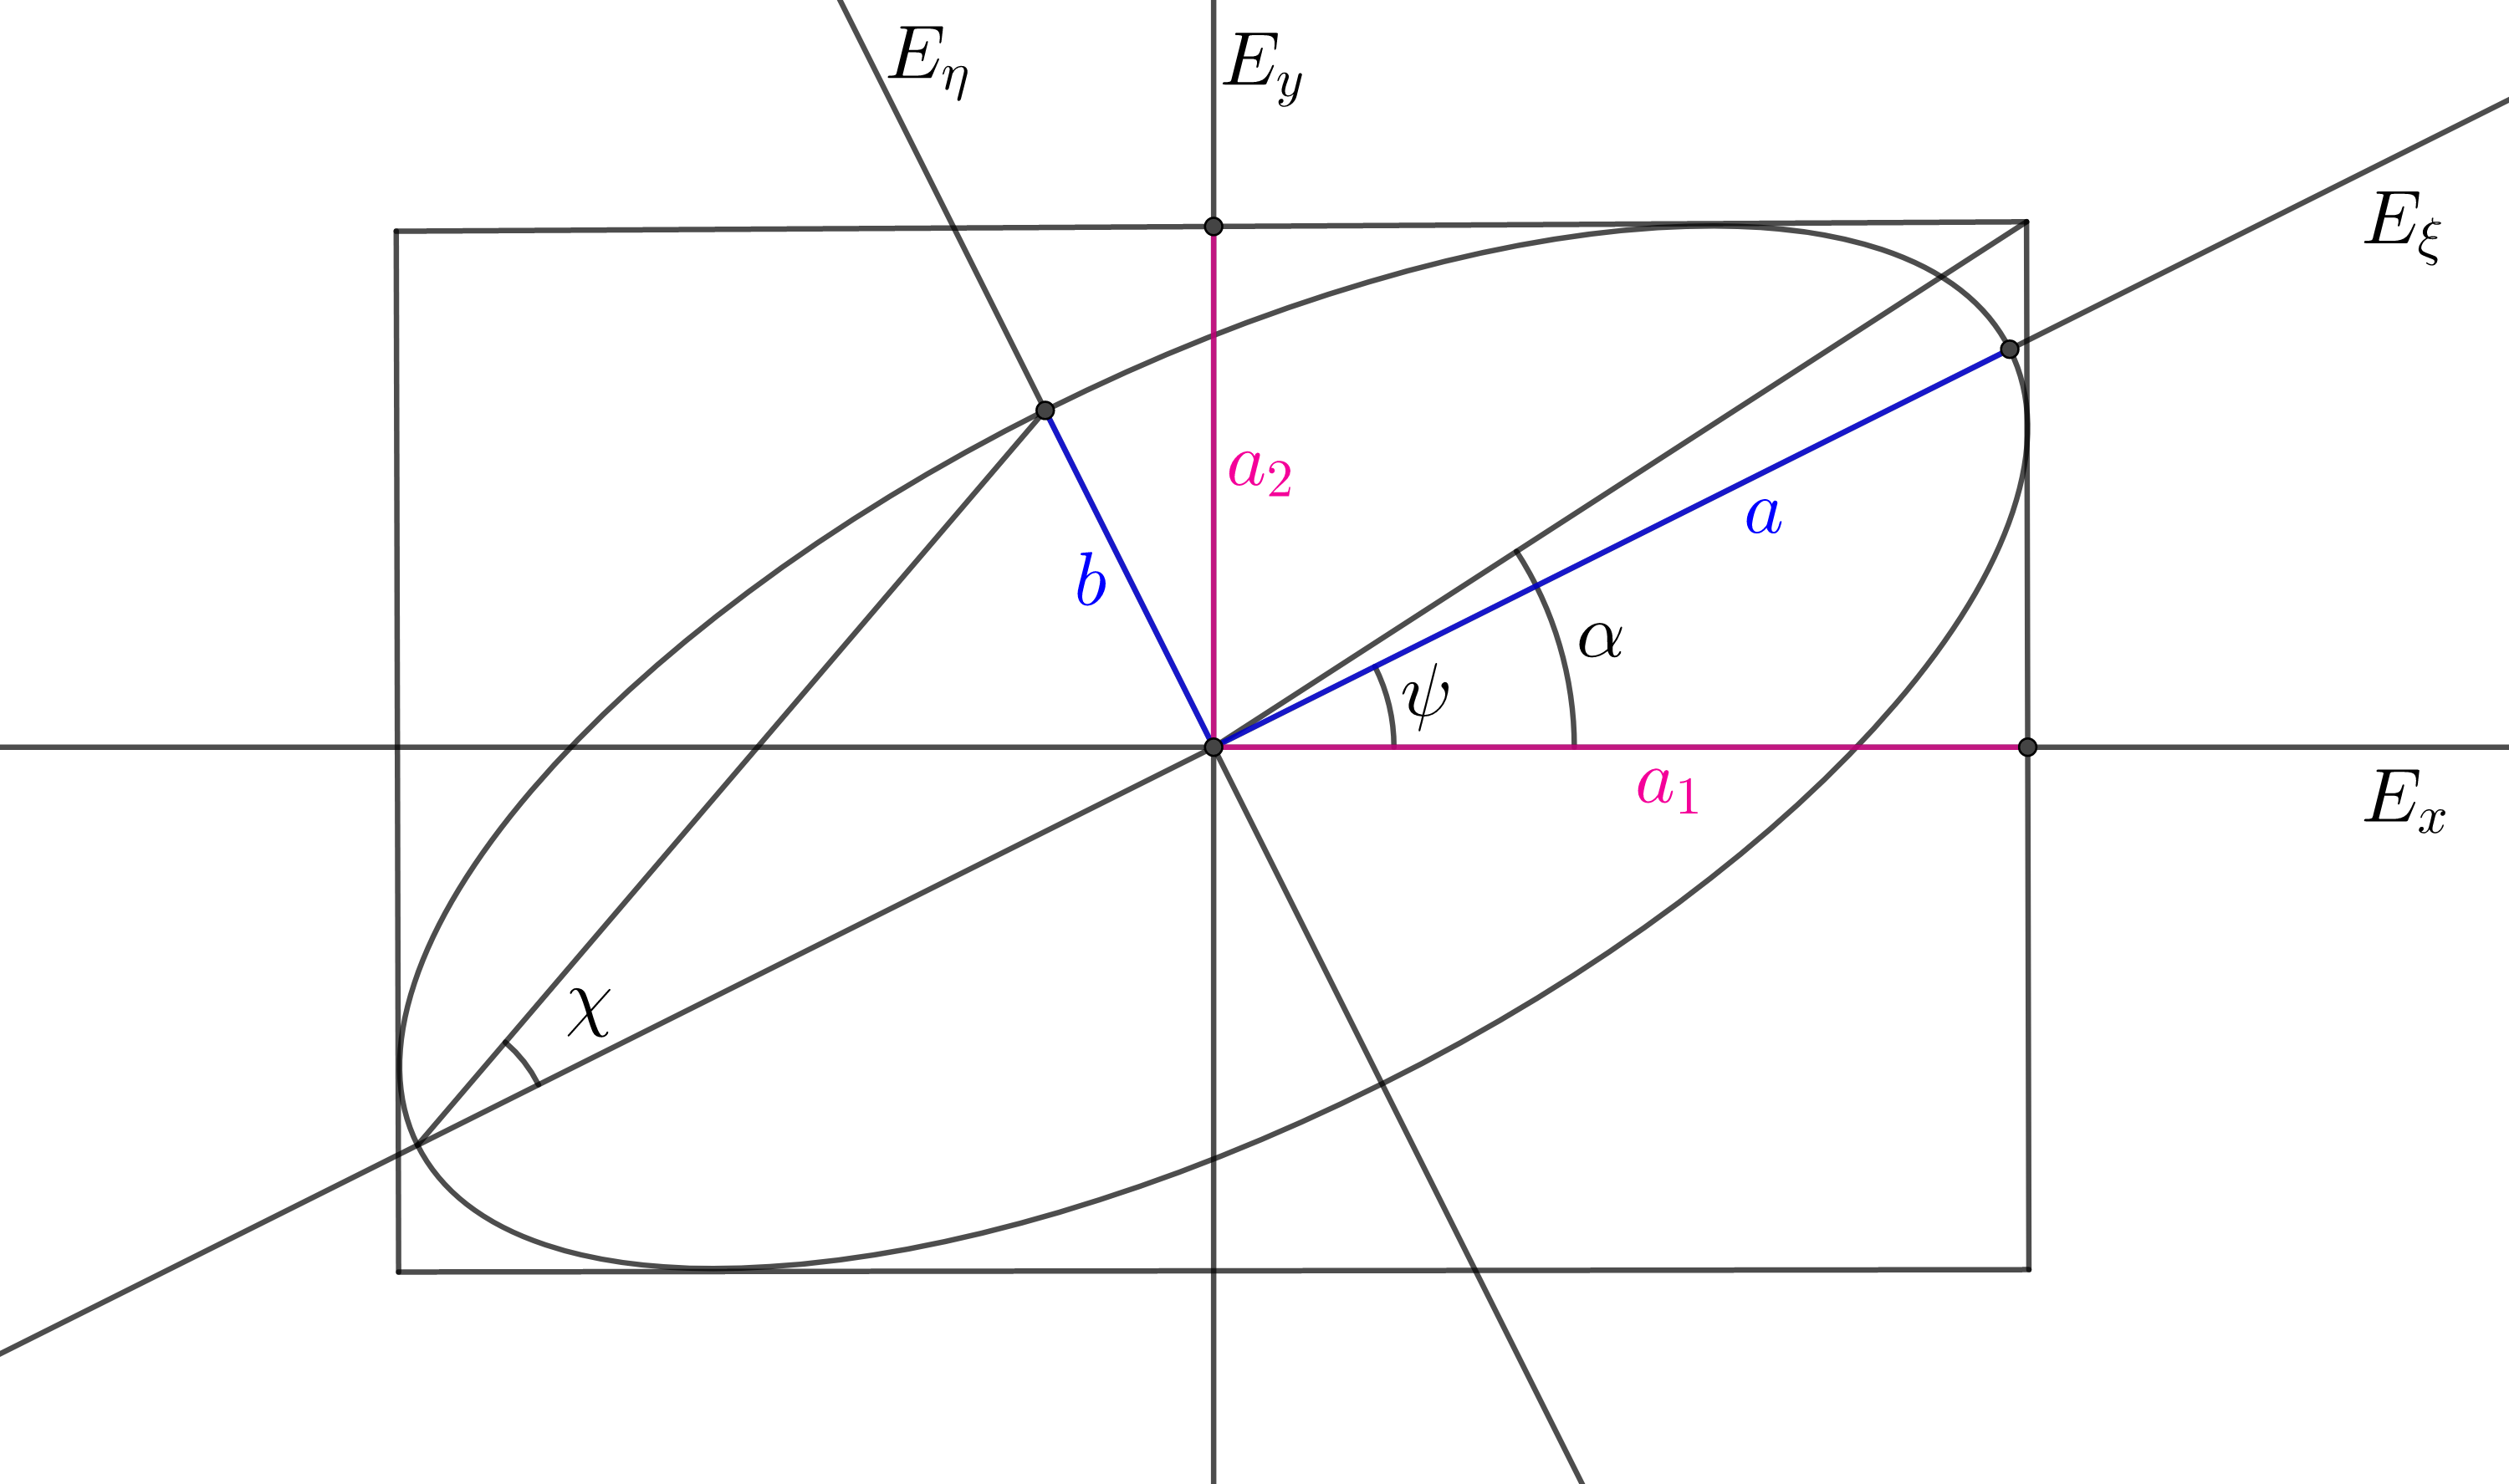
\includegraphics[width=8cm]{ellipse.png}
	\caption{Polarization ellipse}
	\label{fig:pol ellipse}
\end{figure}

Let $\psi$ be the azimuth angle of the ellipse then 
\begin{align}
	\textbf{F}&= R(\psi)\:\textbf{E}\\
	\Rightarrow\begin{bmatrix}E_\xi\\F_\chi\end{bmatrix}&= 
	\begin{bmatrix}
		\cos\psi & \sin\psi \\
		-\sin\psi & \cos\psi
	\end{bmatrix}
	\begin{bmatrix}E_x\\F_y\end{bmatrix}\\
	\Rightarrow
	\begin{bmatrix}
		a \cos(\tau+\delta_0)\\
		\pm b \cos(\tau+\delta_0)
	\end{bmatrix}&=
	\begin{bmatrix}
		\cos\psi & \sin\psi \\
		-\sin\psi & \cos\psi
	\end{bmatrix}
	\begin{bmatrix}
		a_1 \cos(\tau+\delta_1)\\
		a_2 \cos(\tau+\delta_2)
	\end{bmatrix}
\end{align}

We want value of $a, b$, After some tedious calculation \cite{born-wolf}, we reach to some important results, given below 
\begin{align}
	& a^2 + b^2 = a_1^2 + a_2^2\\
	&\pm ab = a_1a_2\sin\delta \label{eq:1.50}\\ 
	&\tan 2\chi \vcentcolon= \pm\frac{b}{a} \label{eq:1.51}\text{ where } \chi\in[-\frac{\pi}{4},\frac{\pi}{4}]\\
	&\tan 2\alpha \vcentcolon= \frac{a_2}{a_1} \text{ where } \alpha\in[0,\frac{\pi}{2}]\\
	&\tan 2\psi = \tan 2\alpha \sin\delta\\
	&\tan 2\chi = \sin 2\alpha \sin\delta
\end{align}
where $\psi$ is the \textit{azimuth} and $\chi$ is \textit{ellipticity} of the polarization ellipse. 

To see the handedness of the rotation of electric field vector in transverse plane,
\begin{enumerate}
	\item[\textbf{Case I}] 
	For right-handed polarization, $\sin\delta>0$, then from equations \ref{eq:1.50}, and \ref{eq:1.51}, we can say 
	$$\tan 2\chi \ge 0\Rightarrow \chi \in \left(0,\frac{\pi}{4}\right]$$
	
	\item[\textbf{Case II}] 
	Similarly for left-handed polarization, $\sin\delta<0$, then from equations \ref{eq:1.50}, and \ref{eq:1.51}, we can say 
	$$\tan 2\chi \le 0\Rightarrow \chi \in \left[\frac{\pi}{4},0\right)$$
\end{enumerate}
	
Now lets calculate the Jones vector of elliptical polarisation,































\subsubsection{Stokes vector and corresponding Poincare representation}
From the eq. \ref{eq:1.16}, we can write for our case, 
\begin{align}
	\boldsymbol{S}= \begin{bmatrix} S_0\\ S_1\\ S_2\\S_3\end{bmatrix} =
	\begin{bmatrix}
		{a_1^2 + a_2^2}\\
		{a_1^2 - a_2^2}\\
		{2a_1a_2\cos\delta}\\
		{2a_1a_2\sin\delta}
	\end{bmatrix}=S_0
	\begin{bmatrix}
		1\\
		\cos 2\chi \cos 2\psi\\
		\cos 2\chi \sin 2\psi\\
		\sin 2\chi
	\end{bmatrix}
\end{align}

So in Poincare sphere representation with axes ${S_1, S_2, S_3}$, the required vector is
\begin{align}
	S_0
	\begin{bmatrix}
		1\\
		\cos 2\chi \cos 2\psi\\
		\cos 2\chi \sin 2\psi\\
		\sin 2\chi
	\end{bmatrix}\longrightarrow
	(S_0\cos 2\chi \cos 2\psi, S_0\cos 2\chi \sin 2\psi, S_0\sin 2\chi)
\end{align}

The evolution of azimuth ($\psi$) and ellipticity ($\chi$) of the polarization state in Poincare representation is shown in the figure \ref{fig:compare poincare}.

\begin{figure}[H]
	\begin{subfigure}[H]{0.48\textwidth}
		\centering
		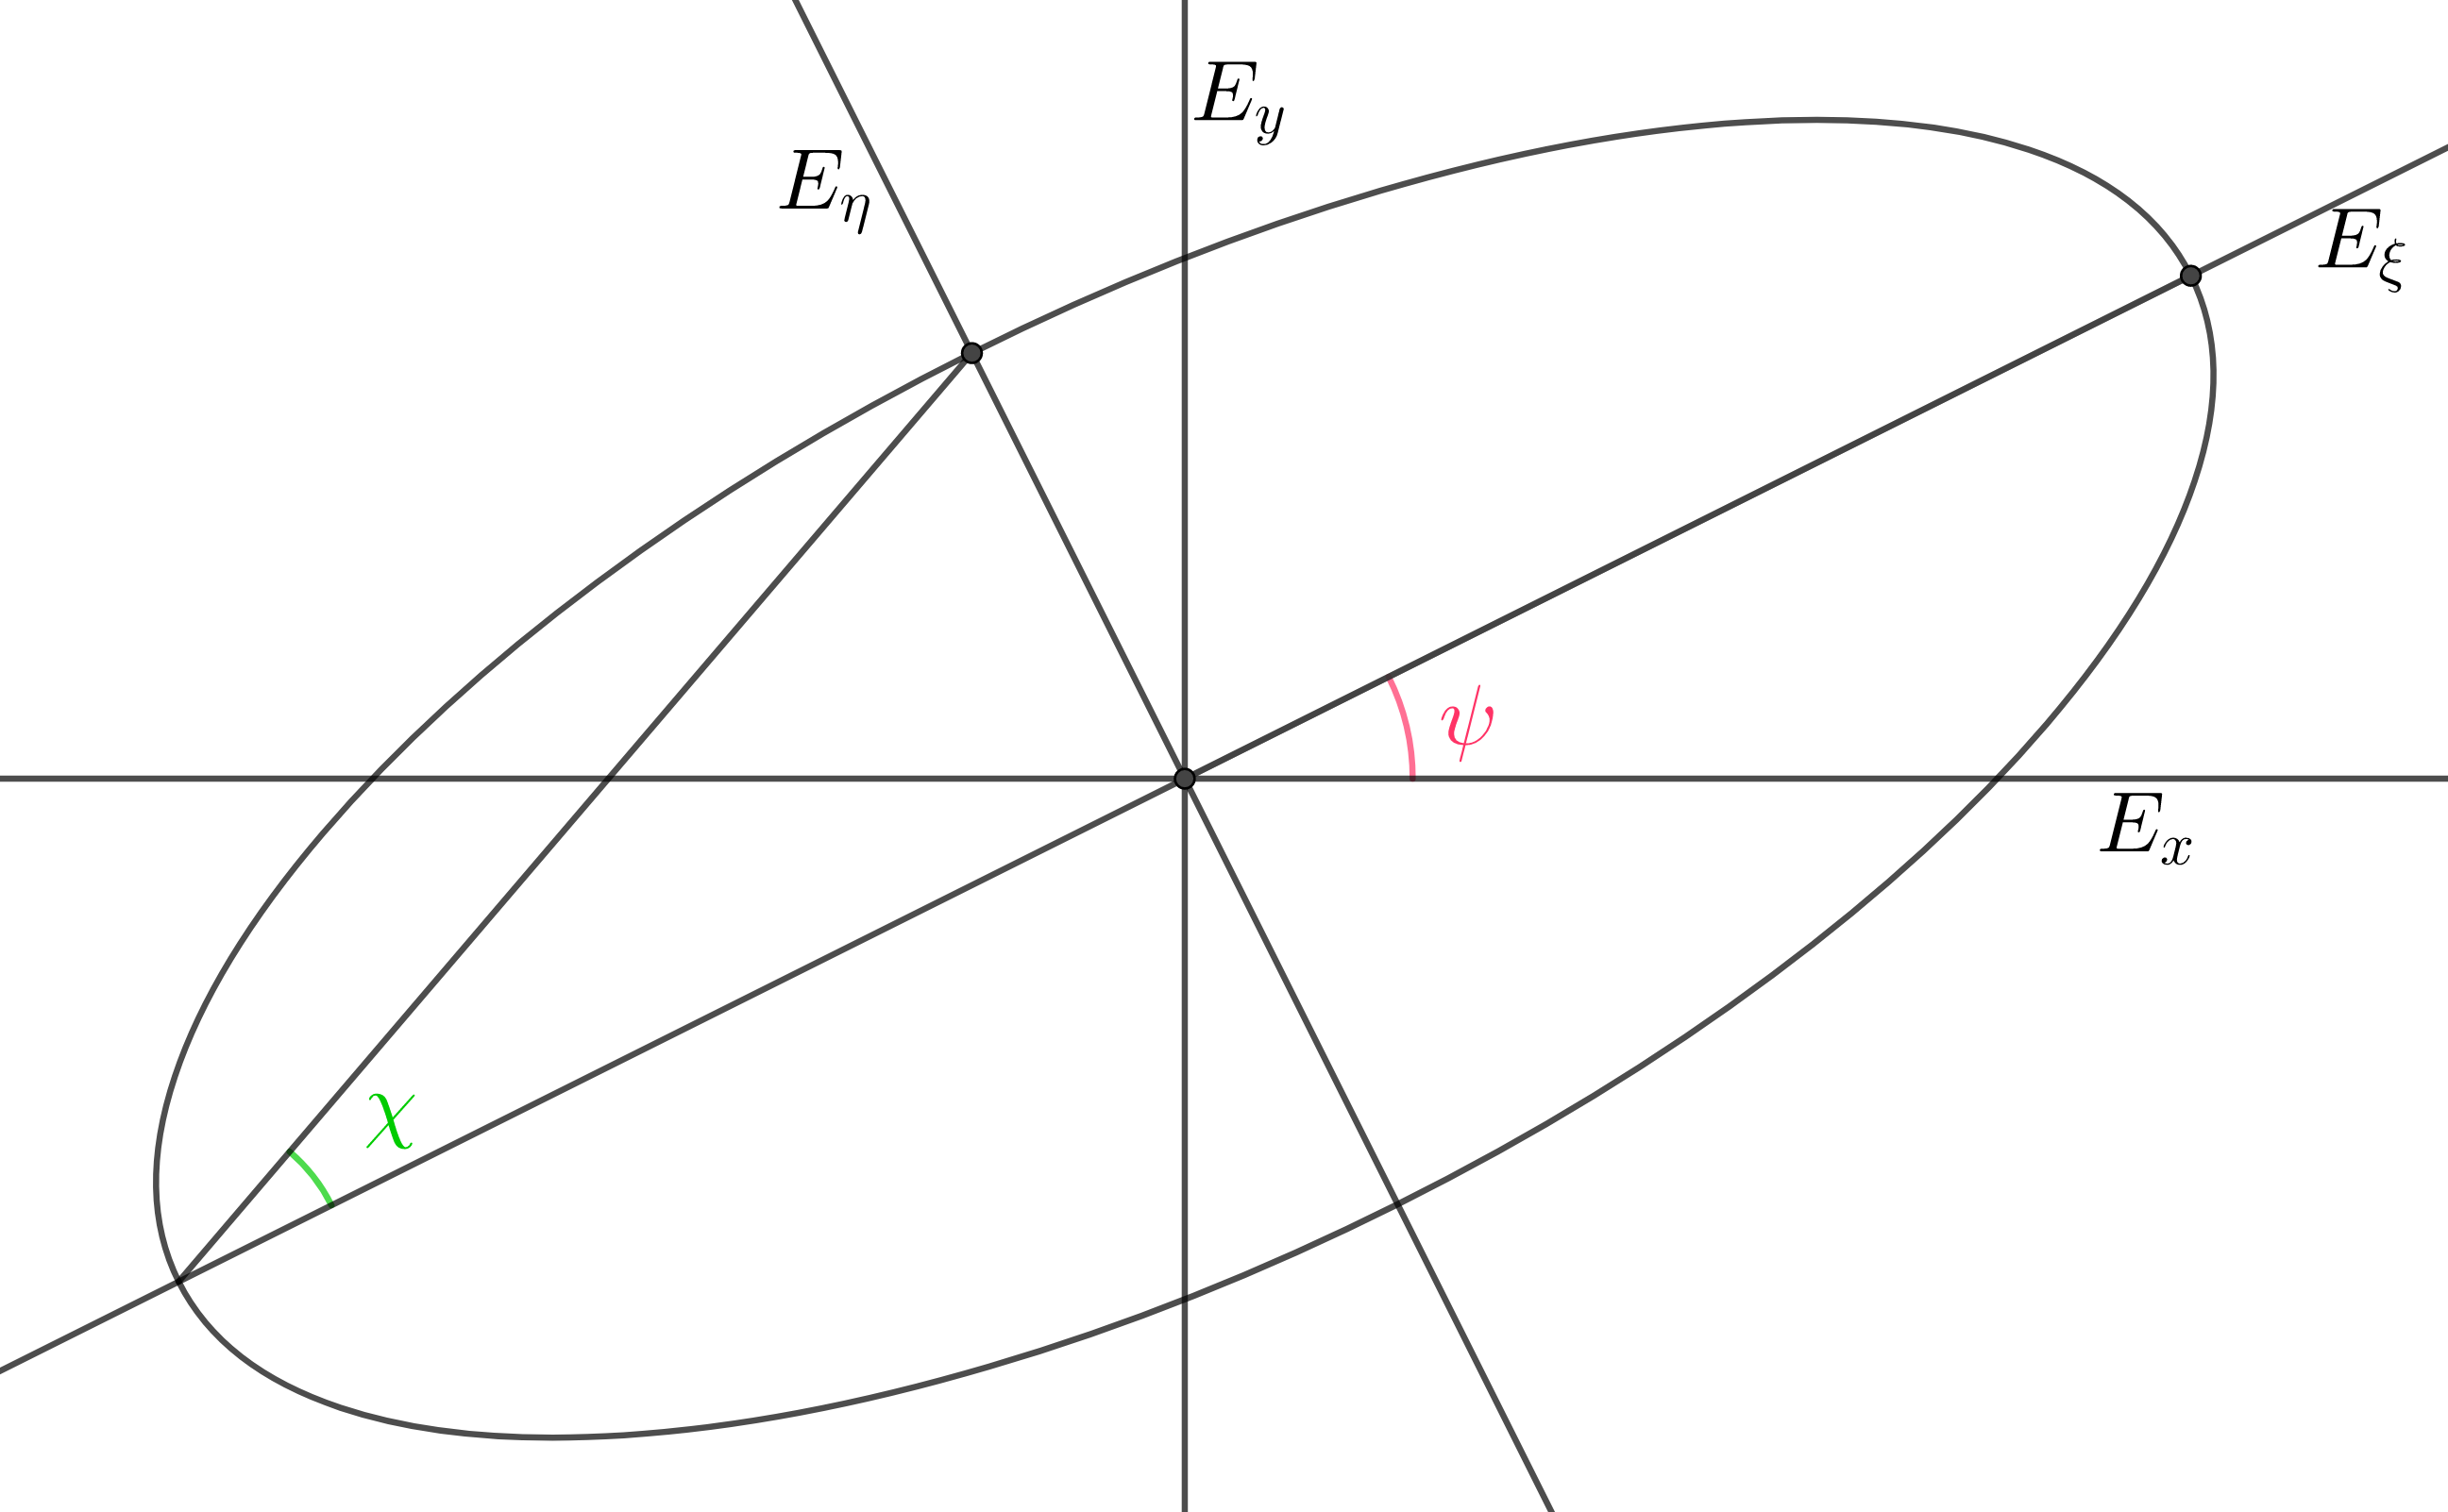
\includegraphics[width=0.9\textwidth]{ellipse_new}
		\caption{}
	\end{subfigure}
	\hfill
	\begin{subfigure}[H]{0.48\textwidth}
		\centering
		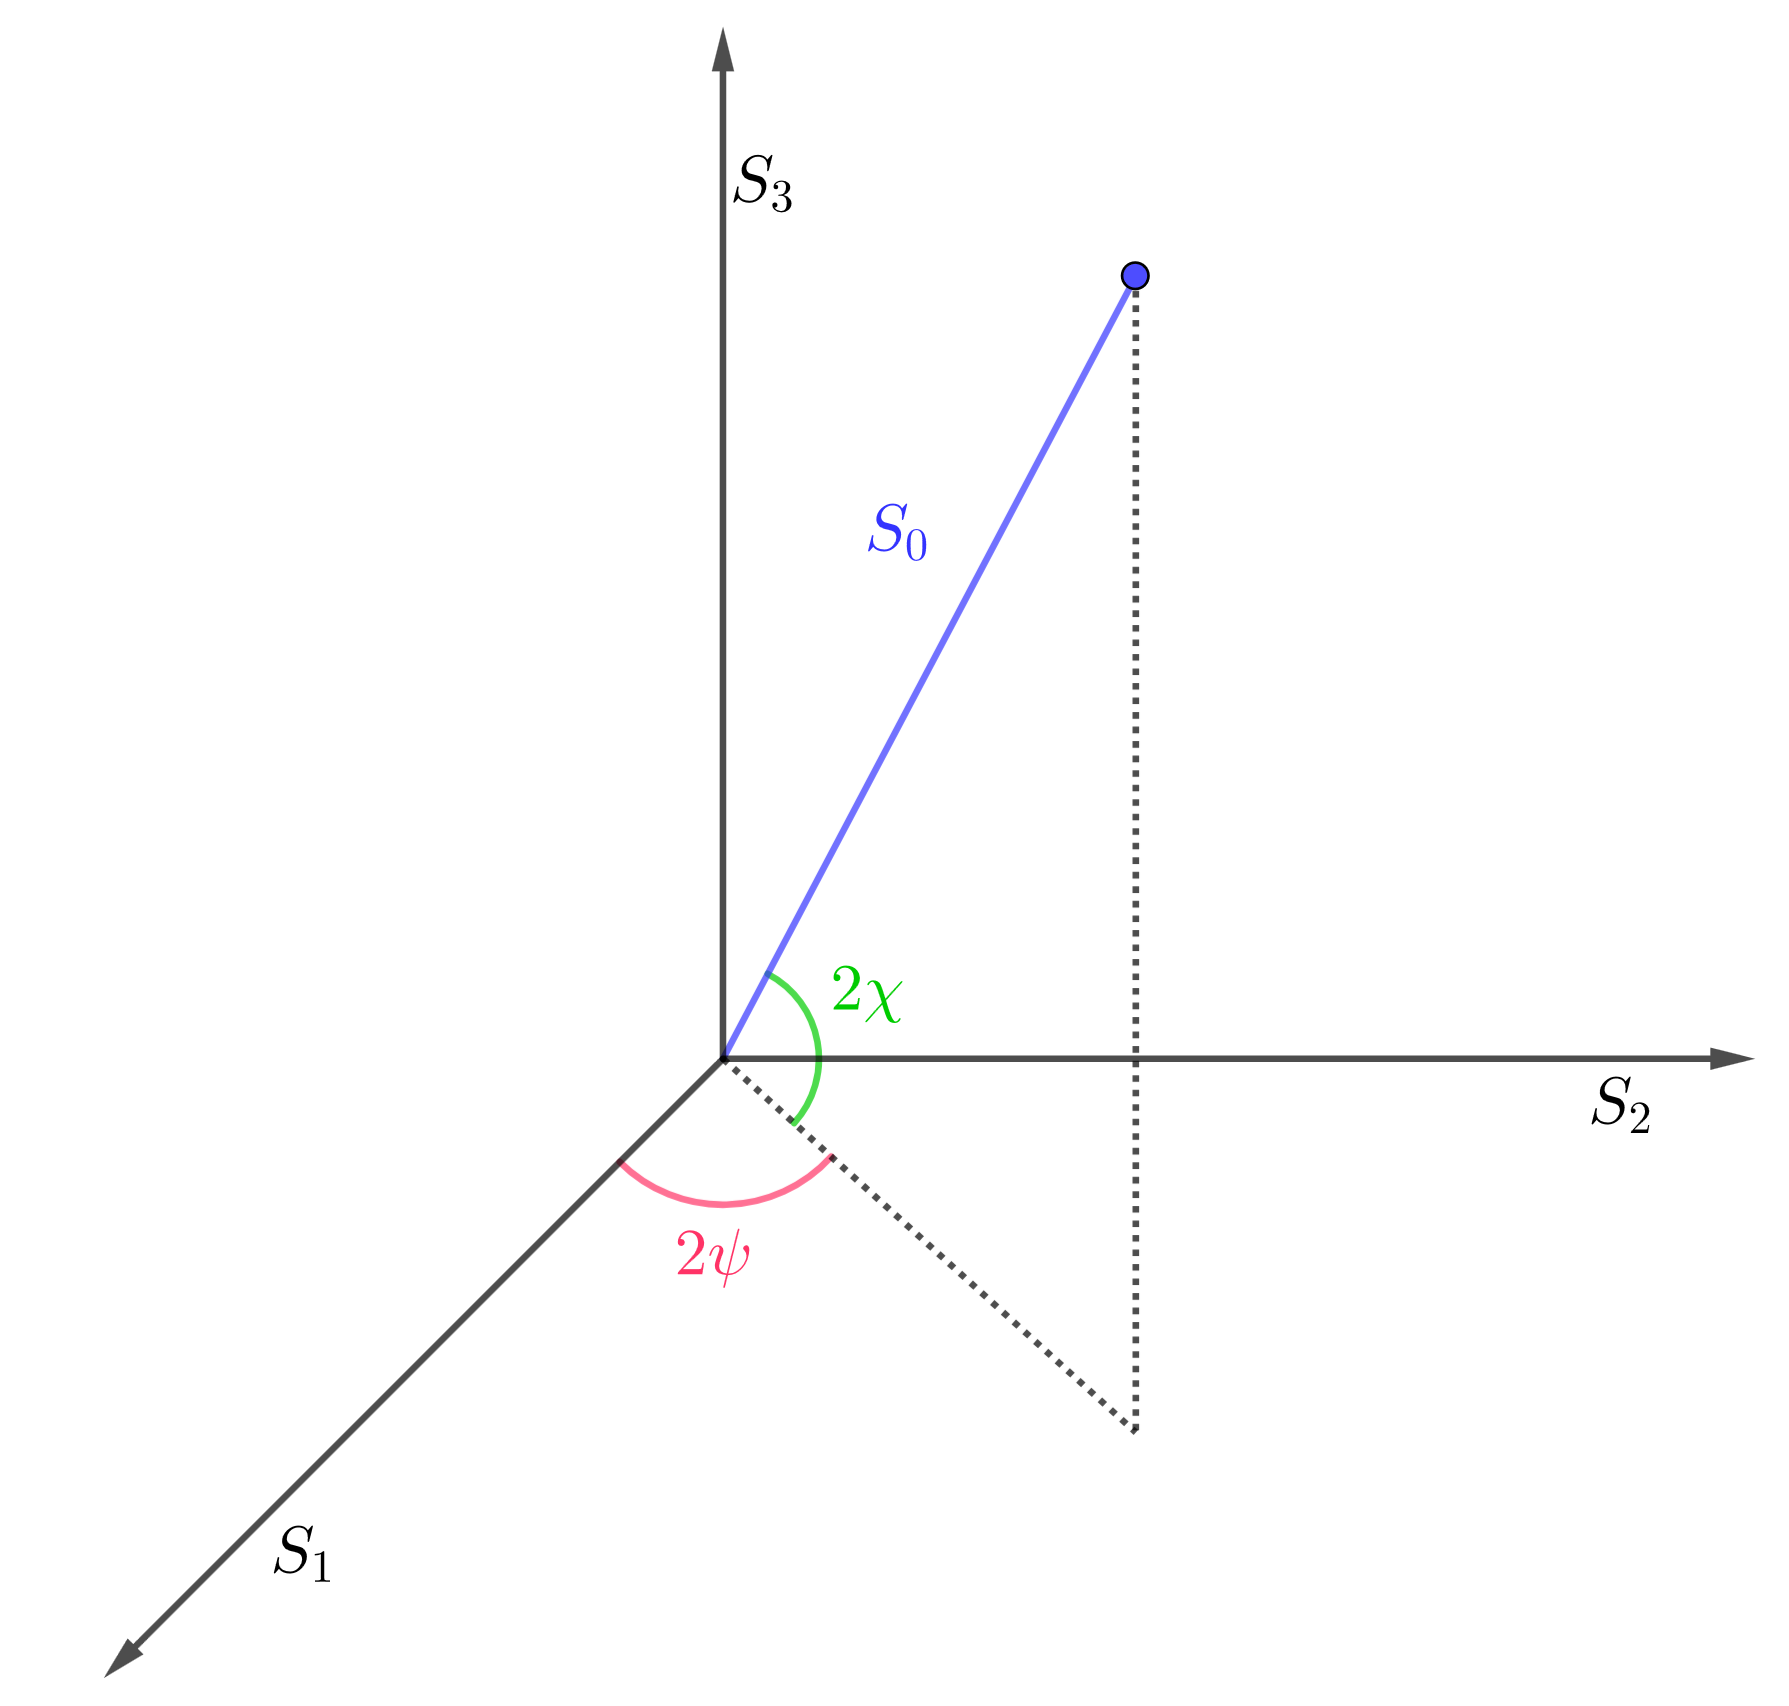
\includegraphics[width=0.7\textwidth]{poincare}
		\caption{}
	\end{subfigure}
	\caption{polarisation ellipse and corresponding Poincare representation}
	\label{fig:compare poincare}
\end{figure}

\begin{thebibliography}{99}
	\bibitem{WO}
	Gupta, S.D., Ghosh, N., \& Banerjee, A. (2015). Wave Optics: Basic Concepts and Contemporary Trends (1st ed.). CRC Press. https://doi.org/10.1201/b19330
	
	\bibitem{born-wolf}
	Born, Max; Wolf, Emil (1999). Principles of optics: electromagnetic theory of propagation, interference and diffraction of light (7th expanded ed.). Cambridge: Cambridge University Press. ISBN 0-521-64222-1. OCLC 1151058062
	
	\bibitem{jones}
	\href{https://en.wikipedia.org/wiki/Jones_calculus}{Jones Calculus - Wikipedia}
	
	\bibitem{coherency}
	Wang Jizhong (1986). A matrix method for describing unpolarized light and its applications. , 2(4), 362–372. doi:10.1007/bf02488478
	
	\bibitem{yt video}
	\href{https://www.youtube.com/watch?v=RowMxWt4mVE&list=LL&index=5}{Polarization (Jones vectors and matrices, partial polarization, Stokes parameters) - YouTube}
	
	\bibitem{stokes}
	Hecht, Eugene (1970). Note on an Operational Definition of the Stokes Parameters. American Journal of Physics, 38(9), 1156–. doi:10.1119/1.1976574     
\end{thebibliography}
%%%%%%%%%%%%%%%%%%%%%%%%%%%%%%%%%%%%%%%%%%%%%%%%%%%%%%%%%%%%%%%%%%%%%%%%%%%%%%%%%%%%%%
\clearpage
\section{GAUSSIAN BEAM}
\subsection{Introduction}
g
\subsection{Parallax wave equaion and solutions}
\subsubsection{Scalar wave solution (without polrisation)}

\subsubsection{Vector wave solution (with polrisation)}

\subsection{Gaussian Beam properties}

\subsection{Differenrt modes of Gaussian beams}

\subsection{Relationship between 1st order LG \& HG beam}

%%%%%%%%%%%%%%%%%%%%%%%%%%%%%%%%%%%%%%%%%%%%%%%%%%%%%%%%%%%%%%%%%%%%%%%%%%%%%%%%%%%%%%
\clearpage
\section{SPIN-ORBIT INTERACTION}
\subsection{Introduction}
soi
\subsection{Angular momentum of Light}

\subsection{Orbital Angular Momentum (OAM)}
\subsubsection{Intrinsic vs Extrinsic OAM}

\subsubsection{OAM of LG Beam}

\subsection{Spin Angular Momentum (SAM)}

\subsection{Spin orbit energy}

\subsection{Geometric phase of light}
\subsubsection{Spin redirection Berry phase}

\subsubsection{Pancharatnam-Berry Phase}

\subsubsection{LG-HG Mode transformation}

\subsection{Types of SOI}

\subsection{SOI in inhomogeneous anisotropic medium}




\end{document}